\chapter{Design \& Implementering}

Dette afsnit beskriver overvejelser omkring valg af design, diagrammer vedrøende implementering

\section{GUI Design}
Da vi skulle lave vores design stod vi mellem to muligheder. Enten skulle det være ren activity baseret eller baseret på en tab menu med få activities. \\
Vi tænkte at det ville være en dårlig bruger oplevelse at man konstant hoppede rundt i activities, og valgte derfor at få med den tab basrede udgave.
Her under ses et billede af hvordan vores Homescreen ser ud i Shine My Room

\begin{figure}[H]
	\centering
	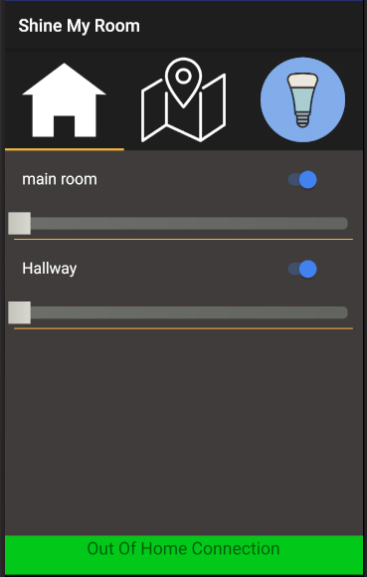
\includegraphics[width=0.5\linewidth, height=0.7\linewidth]{Design/Startscreen}
	\caption{Startscreen}
	\label{fig:Startscreen}
\end{figure}
Applikationen er bygget op af en tab baseret activity hvor der ligger tre tabs man som standard kan hoppe rundt i mellem. Under disse ligger der forskellige fragments som f.eks. listen af rooms som kan ses på billedet. Her kan man se navnet på et af de rum man har oprettede, tænde for pærene som er connected til rummet og bestemme lysstyrken på pærene.


\section{UML diagram}
Her under ses UML diagrammet for Shine My Room
\begin{figure}[H]
	\centering
	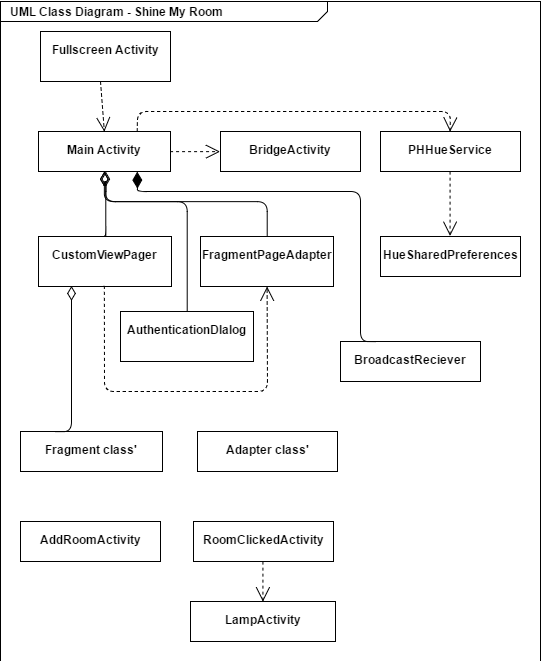
\includegraphics[width=0.6\linewidth, height=0.7\linewidth]{Design/UMLDiagram}
	\caption{UML}
	\label{fig:UML Diagram}
\end{figure}
For at holde UML diagrammet simpelt uden for mange dependencies har vi samlet vores fragment class' og adapter class' i en. \\
Vores fragment class' består altså af klasserne: EditRoomFragment, GeoFencingFragment, LoadingFragment, NoBridgeConnectFragment og RoomListFragment.\\
Adapter class' består af: AddRoomAdapter, EditRoomAdapter, FragmentPageAdapter, RemoteRoomAdapter, RoomAdapter og RoomClickedAdapter.

De activities som ligger i bunden er lagt ind på denne måde, da de udspringer af en fragment, og derfor kunne vi ikke placere deres dependensy pga den samlede fragment class.
\newpage

\section{Sekvensdiagram}
Her under ses sekvensdiagrammet for Use Case 1 for Shine My Room
\begin{figure}[H]
	\centering
	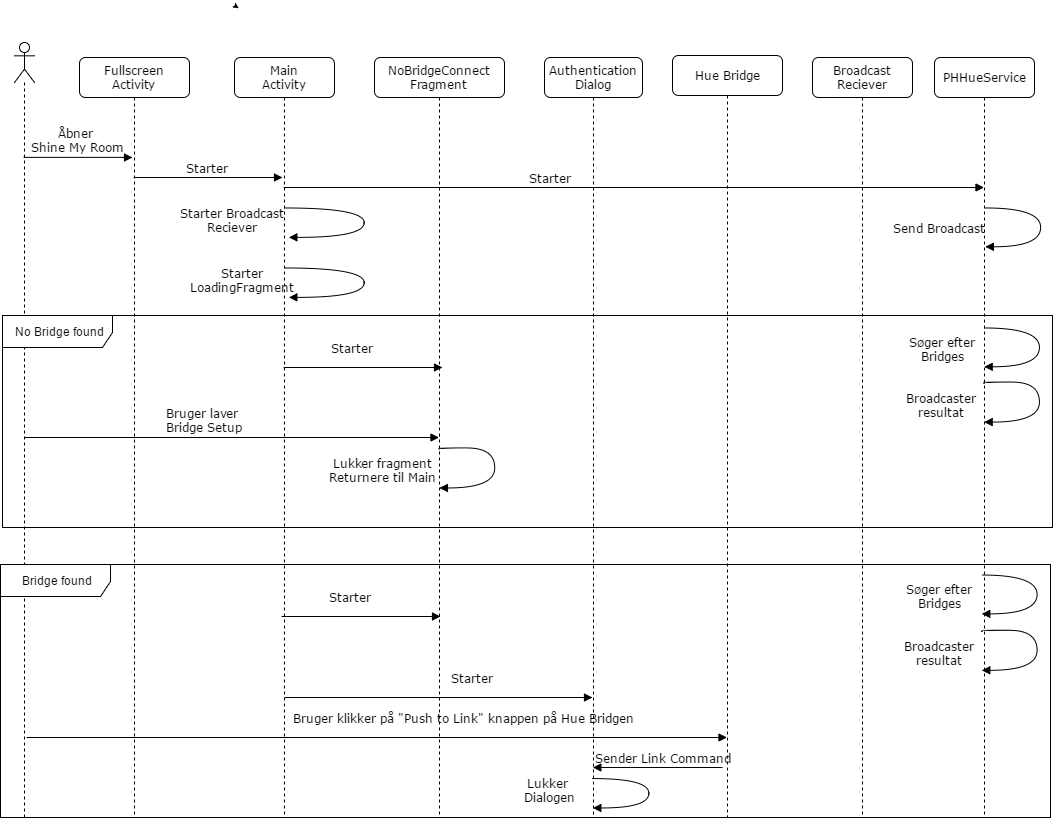
\includegraphics[width=1\linewidth, height=0.8\linewidth]{Design/SekvensDiagramUC1}
	\caption{Sekvensdiagram Use Case 2}
	\label{fig:SekvensdiagramUC1}
\end{figure}
Sekvensdiagrammet ovenfor viser brugerens og applikationens logik når man skal connecte til en Hue Bridge. \\
Her bliver der taget højde for vores PHHueService kan lokalisere end Hue Bridge i nærheden eller ej, og hvad brugeren så skal fortage sig for at komme videre i begge tilfælde.
\newpage

Her under ses sekvensdiagrammet for Use Case 2 for Shine My Room
\begin{figure}[H]
	\centering
	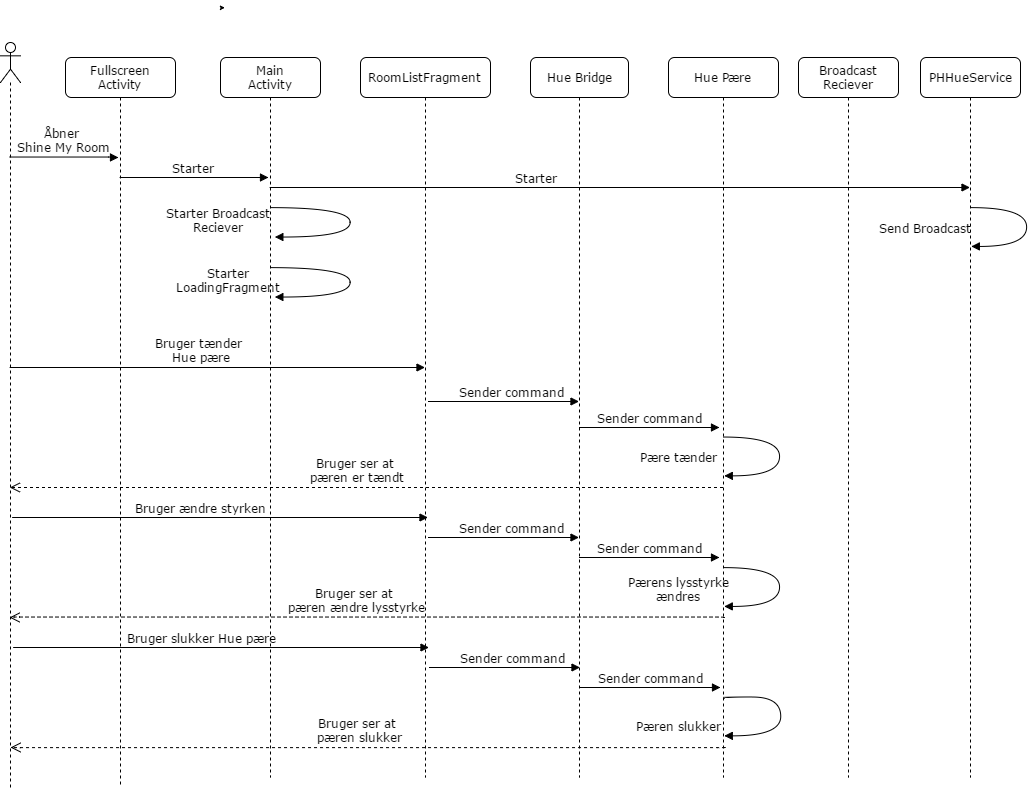
\includegraphics[width=1\linewidth, height=0.8\linewidth]{Design/SekvensDiagramUC2}
	\caption{Sekvensdiagram Use Case 2}
	\label{fig:SekvensdiagramUC2}
\end{figure}
På sekvensdiagram ovenfor kan det ses hvordan at det meste sker meste gennem MainActivity. Brugeren interagere med RoomListFragmentet for at lave ændringer ved Hue pærene. RoomListFragment ligger i MainActivity, men for at vise at der ligger en fragment list i MainActivity har vi lavet det på denne måde, da det er fragmentet der indeholder funktionaliteten til ændringerne. \\

\section{Afgrænsning}
Vi har mulighed for at tænde og slukke pærene og styre lysstyrken af pæren. Det lykkedes os dog ikke at få lavet så man kunne skifte farven, da The C.I.E. Color Space tager noget længere tid at sætte sig ind i, end vi først lige havde antaget.\\
Et andet af de større problem vi løb ind i var når vi ønskede at tilføje og redigere i rooms. Vi havde store problemer med at få Hue API'et til at arbejde sammen med os når vi ønskede at lave ændringer og ikke bare læse værdier fra Hue Bridgen.
